\section{Circuito: Amplificador sumador inversor}

El siguiente circuito es un un sumador. Debe ser diseñado para las condiciones de contorno especificadas más abajo.

\begin{figure}[h!]
    \centering
    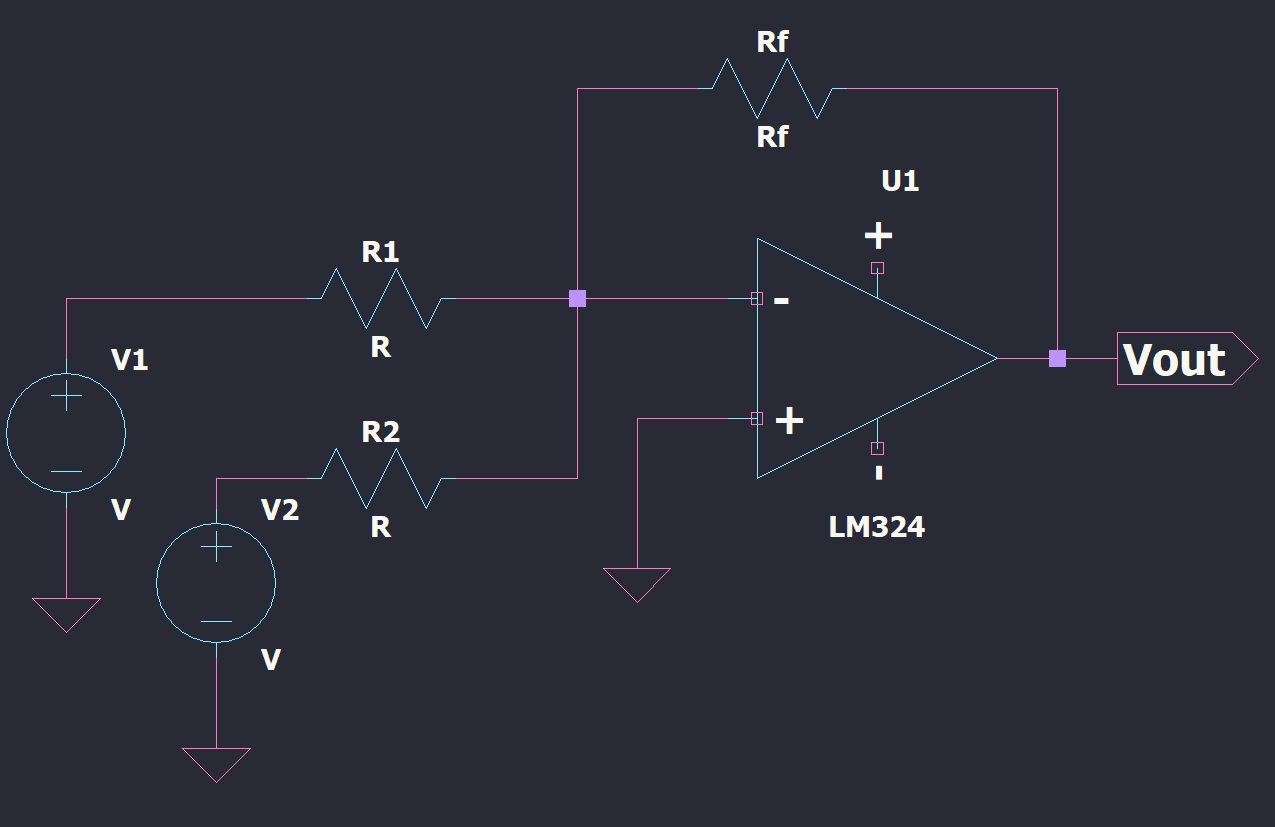
\includegraphics[width=0.90\linewidth]{img/esquematico_complete.png}
    \caption{Esquemático del circuito N° 1}
    \label{fig:esquematico_complete}
\end{figure}

\begin{itemize}
  \item Tipo de amplificador operacional: LM324
  \item Alimentación: $Vcc = 10V, Vss = -10V$
  \item Ganancia en banda media: $A = \frac{V_O}{V_1} = \frac{V_O}{V_2} = 30$
  \item Impedancia de entrada: $Z_i$ del amplificador no puede alterar o cargar la fuente de señal, es decir, $R_i  \ll Zi_1$ y $Zi_2$ (al menos 10 veces)
  
  \item Resistencias: Usar Resistencias $<= 1M \Omega$
  \item Condiciones de las fuentes: Las fuentes V1 y V2 deben considerarse en las condiciones 1.A y 1.B

\end{itemize}





\section{Analisis del circuito}

\subsection{Vo = f(V1,V2)}

Este circuito tiene dos entradas, V1 y V2. 
La salida del circuito es la suma de las dos señales de entrada, amplificada. Para eso realizaremos el análisis haciendo uso del teorema de superposición nos permite calcular la respuesta de un circuito a dos o más señales de entrada, sumando las respuestas individuales a cada señal de entrada.

En este caso, podemos aplicar el teorema de superposición para calcular la salida del circuito como la suma de las salidas, considerando $V_2=0$ y luego considerando $V_1=0$. Para ambos casos podemos observar que tenemos un amplificador en configuración inversor. Por lo tanto considerando AO ideal: 

\vspace{1em}

Para el caso en el que pasivamos la fuente de tensión $V_2 = 0$ la tensión de salida es :

\[V_{01} = - \frac{R_f}{R} \cdot V_1 \]

Luego el caso en el que pasivamos la fuente de tensión $V_1 = 0$ obtenemos una tensión de salida:

\[V_{02} = - \frac{R_f}{R} \cdot V_2 \]

Aplicando el teorema, sumamos ambas salidas obtenemos:

\[V_{0} = V_{01} + V_{02} = - \frac{R_f}{R} \cdot (V_1 + V_2) \]

\vspace{1em}

\subsubsection{Ganancia del lazo: T}
Para calcular la ganancia T, primero pasivamos las fuentes de entrada y se abre el lazo, quedando así el siguiente circuito para analizar;

\begin{figure}[h!]
    \centering
    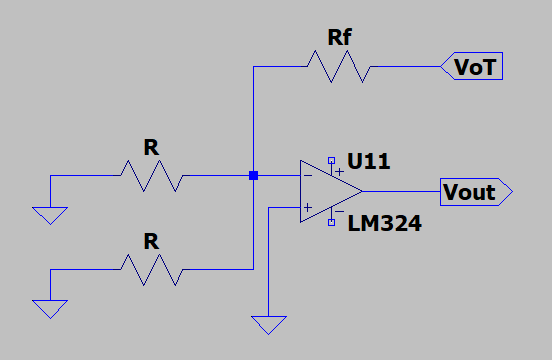
\includegraphics[width=0.90\linewidth]{img/equivalente_lazo.png}
    \caption{Circuito equivalente para el lazo}
    \label{fig:equivalente_lazo}
\end{figure}


\[T = \left.\frac{V_{o}}{V_{oT}}\right|_{V_{1}=V_{2}=0} = \frac{V_{o}}{V^{-}} \cdot \frac{V^{-}}{V_{2}} = (-A_d) \frac{(R // R)}{(R // R)+R_f} \]
\[
 T (s) = -Ad(s) \cdot \frac{\frac{R \cdot R}{R+R}}{\frac{R \cdot R}{R+R} + R_f} = ... 
 = -A_d (s) \cdot  \frac{R}{R + 2\cdot R_f}\] 

\subsection{Errores DC}

\subsubsection{Error de corriente de offset: Ios}
Para calcular las corrientes de offset, se pasivan las fuentes y el circuito queda de esta manera:

\begin{figure}[h!]
    \centering
    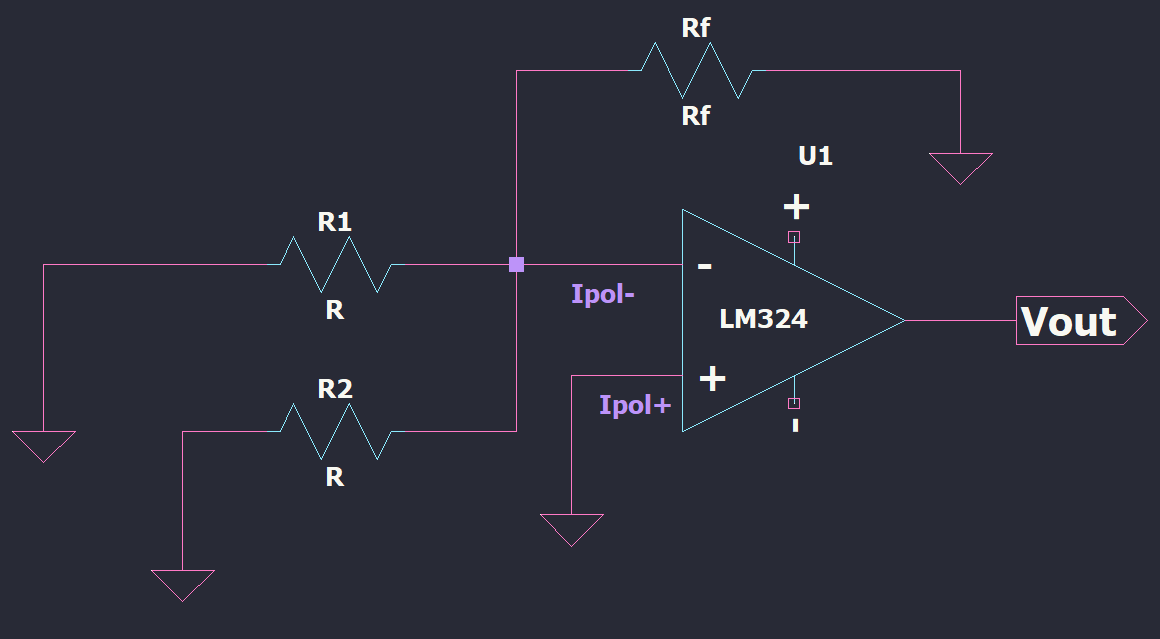
\includegraphics[width=0.90\linewidth]{img/equivalente_ios.png}
    \caption{Circuito equivalente para calcular el error debido a Ipol}
    \label{fig:equivalente_ios}
\end{figure}

\vspace{1em}
Calculamos por partes la ganancia entre la salida y las distintas corrientes de polarización. A continuación se tiene el error debido a la $I_{pol}^{+}$.

\[
\left.\Delta V_{o} \right|_{I_{p o l}^{+}}= I_{p o l}^{+} \cdot R^{+} = 0
\]
Debido a que no hay ninguna impedancia conectada a la entrada no inversora, el error debido a  $I_{pol}^{+}$ es cero.

\vspace{1em}

Luego se tiene el error a lazo abierto debido a la $I_{pol}^{-}$.
 
\[
\left.\Delta V_{o} \right|_{I_{pol}^{+}} = I_{pol}^{-} \cdot (-A_d) \cdot (-R_f // R // R)
\] 

\[\left.\Delta V_{o} \right|_{I_{pol}^{+}} 
= I_{pol}^{-} \cdot (-A_d) \cdot \frac{1}{\frac{1}{R_f}+\frac{1}{R}+\frac{1}{R}} 
= ... = I_{pol}^{-} \cdot A_d \cdot \frac{R_f R}{(R+2 R_f)} \] 
 
Luego si calculamos el error debido a la corriente de offset a lazo cerrado, obtenemos:

 \[ \Delta V_{o_{LA}} = \left.\Delta V_{o} \right|_{I_{pol}^{+}} - \left.\Delta V_{o} \right|_{I_{pol}^{-}}  \] 



\[
\Delta V_{o}= \frac{A_d \frac{R_f R}{(R+2 R_f)} I_{pol}^{-}}{1 - T} 
= \frac{A_d \frac{R_f R}{(R+2 R_f)} I_{pol}^{-}}{1 + A_d \frac{R}{2 R_f+R}} 
= ... =  \frac{Ad \cdot  I_{pol}^{-} \cdot R \cdot R_f}{Ad \cdot R + R + 2 \cdot R_f} 
\] 

Luego  tomando la ganancia ideal del AO $\left(A_{d} \rightarrow \infty\right)$ se cancelan términos y el resultado es:

\[
\Delta V_{o} 
= I_{pol}^{-} \cdot R_f
\]


\subsubsection{Tensión de Offset: Vos}
 
Para el análisis de este error se utiliza el circuito de la figura \ref{fig:equivalente_vos}. 


\begin{figure}[h!]
    \centering
    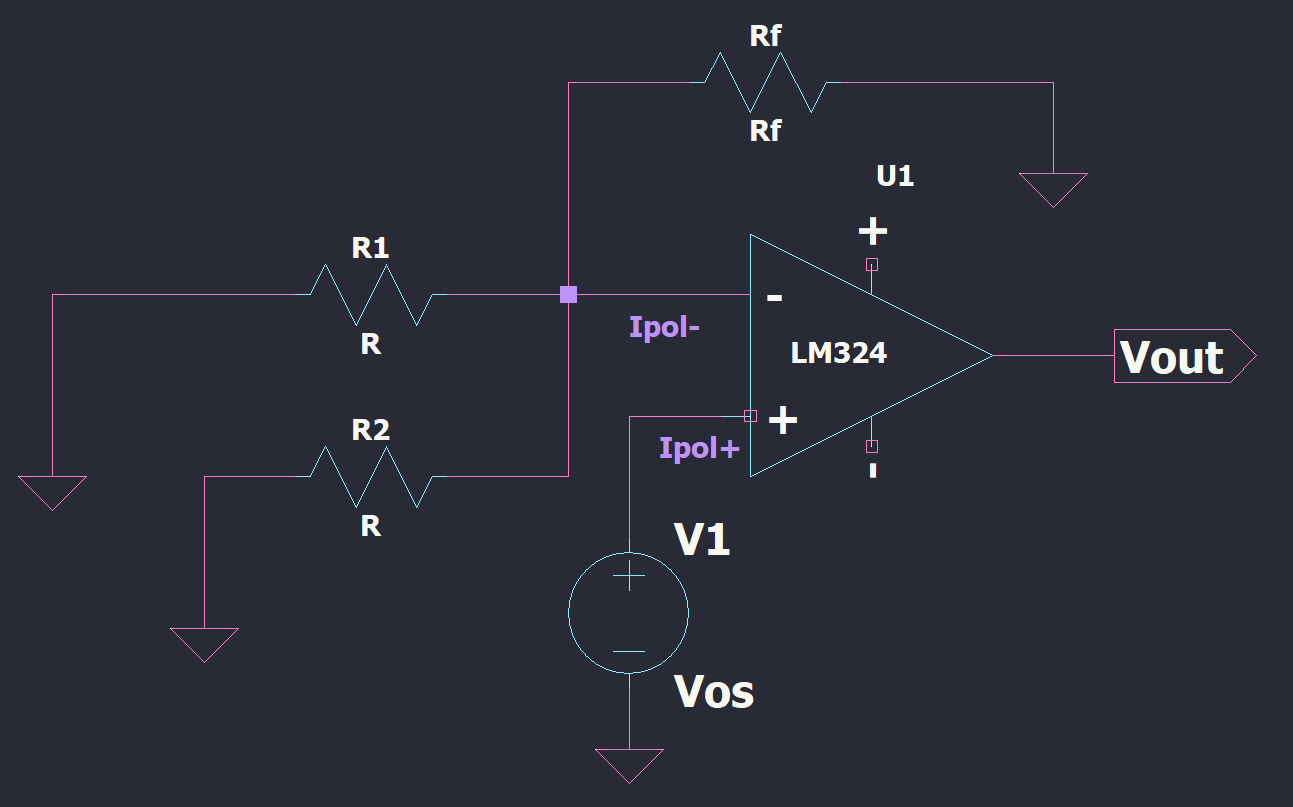
\includegraphics[width=0.90\linewidth]{img/equivalente_vos.png}
    \caption{Circuito equivalente para calcular Vos}
    \label{fig:equivalente_vos}
\end{figure}

Se calcula la ganancia de tensión a lazo abierto entre el error $V_{os}$ y la salida.

\[
A_{vos} = \left.\frac{V_{o}}{V_{o s}}\right|_{LA} = 
\frac{V_{o}}{V^{+}} \cdot \frac{V^{+}}{V_{os}} = A_d
\]

Luego si aplicamos black, para obtener el error, se tiene:
 
\[
\Delta V_{os} = \frac{A_d \cdot V_{os}}{1+A_d \frac{R}{2 R_f+R}} = ... 
 = \frac{A_d \cdot V_{os} \cdot (R + 2 \cdot R_f)}{A_d \cdot R + R + 2 \cdot R_f}
\]
 

Como se toma que el amplificador es ideal la ganancia es ideal $\left(A_{d} \rightarrow \infty\right)$ es entonces que se tiene:

\[
\Delta V_{os}  = V_{os} \cdot \frac {R + 2 \cdot R_f}{R} 
=  V_{os} \cdot (1 + 2 \cdot \frac {R_f}{R} )
\]
 
\subsubsection{Ad \texorpdfstring{$< \infty$}{< ∞}}

Debido a que en la realidad $A_d$ es menor a infinito, debemos considerar el error que aporta.

\[ A_v(s) = \left.\frac{V_0}{V_{1,2}}\right|_{V_{oT} = 0}  = -A_d(s) \cdot \frac{R_f}{R + R_f} = -A_d(s) \cdot (1 - K) \]

\[ T(s) = \left.\frac{V_0}{V_{oT}}\right|_{V_{1,2} = 0} = -A(s) \cdot  \frac{R}{R + 2\cdot R_f}= - A_d(s) \cdot K \]

\[ A_{vf}(s) = \frac{A_d(s)}{1 + K A_d(s)} = \frac{ \frac{1}{K} }{1+\frac{1}{K\cdot A_d(s)}}  \]

\[A_{vf}(s) = \frac{A_{vfi}}{1 - \frac{1}{T(s)}}  \quad  \text{con}  \quad  \epsilon_{G(A_d)} = \frac{1}{T} \]


Luego tenemos que:
\[
\epsilon_{G(A_d)} = \frac{(V_{ideal} - V_{real})}{V_{oi}} = \frac{\Delta V_0}{V_{oi}} \quad \rightarrow \quad \Delta V_0 = \epsilon_{G(A_d)} \cdot V_{oi}  
\]



\[
\Delta V_0 = \epsilon_{G(0)} \cdot V_{o\text{max}} 
\]

Si reemplazamos obtenemos que:

$$
\Delta V_{o}=\frac{F.S}{\left|T_{o}\right|}
$$


\subsubsection{RRMC \texorpdfstring{$< \infty$}{< ∞}}

Como la entrada no inversora del amplificador se encuentra directamente conectado a masa el error debido a la RRMC resulta despreciable:

\[ \Delta V_{o (RRMC) }=0 [ mV ]\]


\subsection{Errores AC}

\subsubsection{Ancho de banda de pequeña señal \texorpdfstring{$f_H$}{fH}}



Ancho de banda de pequeña señal $\left(w_{h}=-3[d B]\right)$

Observando la hoja de datos del amplificador LM324, obtenemos que:
\[f_T = 1 [MHz]\]
 

Luego, sabiendo que el ancho de banda en pequeña señal se puede calcular con la siguiente formula: 
\[ W_H = W_{T} K \]

De donde K es:
\[ K=\frac{R}{R+2 R f}\]

Por lo tanto, reemplazando en la fórmula general,

\[ w_H = w_{T} \cdot \frac{R}{R+2 R_f} \]


\subsubsection{Ancho de banda a plena potencia \texorpdfstring{$f_{HP} (10 V_{pap})$}{fH(10Vpap)} }

Primero obtenemos el Slew Rate, que se refiere a la velocidad máxima a la que el amplificador operacional puede cambiar su salida cuando hay un cambio en la entrada. Se mide como voltaje relativo al tiempo, y la unidad típica utilizada en las hojas de datos es voltios por microsegundo (V/µs):


 \[ S R=0,5[V / \mu S] \] 

Luego, se utiliza la siguiente fórmula para conocer el valor de $f_{Hp}$, despejando de la misma $\omega_{Hp}$.

\[ S R = \omega_{Hp} \hat{V}_{o} = 2 \pi \cdot  f_{1} \cdot  \hat{V}_{o} \]

Es entonces que reemplazando se tiene:
\[ f_{Hp} = \frac{S R}{2 \pi \hat{V}_{o}} = \frac{0.5[V/ \mu \mathrm{S}]}{2 \pi 10[V]} \]
\[ f_{Hp} = 7,957 [\mathrm{kHz}] \]

\subsubsection{Error vectorial }

Primero obtenemos la ganancia normalizada, que se calcula dividiendo la ganancia a lazo cerrado sobre la ganancia a lazo cerrado ideal (sin variación con la frecuencia):

\[ a_{vf} = \frac{A_{vf}}{A{vfi}} = \frac{1}{1 + \frac{s}{\omega_h}} \]

Luego expresamos su modulo y su fase:

\[ |avf| = \frac{1}{\sqrt{\omega^2_s + 1}} \]


\[ \phi = -atan\left(\frac{\omega}{\omega_h}\right) \]

Con estas definiciones, obtenemos el error vectorial:

\[ \varepsilon_v = \frac{a_{vf}} - 1 \]

Y expresamos en términos de modulo y fase:

\[ |\varepsilon_v| = 1 - \frac{1}{\sqrt{\left(\frac{\omega}{\omega_{h}}\right)^2 + 1}} \]

\[ \phi_v = -\arctan\left(\frac{\omega}{\omega_h}\right) + \frac{\pi}{2} \]


\subsubsection{Tabla de error vectorial normalizado}


\subsubsection{Máxima excursión}
El valor máximo de excursión se obtiene dividiendo el fondo de escala sobre la ganancia media:

\[ V_{max}=\frac{F S}{Avfm} =  \pm 0.33[ V ] \]




\subsection{Resumen}

\[V_{0} = V_{01} + V_{02} = - \frac{R_f}{R} \cdot (V_1 + V_2) \]
\[T (s) = -A_d (s) \cdot  \frac{R}{R + 2\cdot R_f}\]


Errores DC

\[ \Delta V_{ios} = I_{pol}^{-} \cdot R_f \]
\[ \Delta V_{os}  = V_{os} \cdot (1 + 2 \cdot \frac {R_f}{R} )\]
\[ \Delta V_{o (Ad)}=\frac{F.S}{\left|T_{o}\right|}\]
\[ \Delta V_{o (RRMC) } = 0 [ mV ]\]
 
Ancho de banda:

\[ w_H = w_{T} \frac{R}{R+2 R_f} \]

\[ f_{Hp}=7,957[\mathrm{kHz}] \]
 

